\documentclass[]{article}

\usepackage{xltxtra}
\usepackage{rotating}
\usepackage{graphicx}
\usepackage[xetex, breaklinks=true, hyperfootnotes=false, hyperfigures=false, colorlinks=true]{hyperref}
\usepackage{fontspec}

\title{Notes on the dictionary approach, and some tests of a new method}
\author{Chris Forstall}

\date{2012-03-08}

\begin{document}
	
	\setmainfont{Arial}
	
	\maketitle


	\begin{abstract}
		
		Jeffrey Rydberg-Cox confirms that our Dictionary Approach is on the right track.  The methods we use are very similar to a system he used with some success, not only in detecting Latin synonyms, but also in cross-linguistic matching.

		Here are some preliminary results from a slightly new take on the Dictionary Approach, namely, using topic modelling on the dictionary.  It makes use of the Whitaker's Words dictionary rather than the Perseus Lewis and Short.  Results are compared to a random set of synonyms taken from a printed 19th-century Latin thesaurus, and are intriguing, but not yet reliable.

	\end{abstract}

	\section{Current methods: comparandum and positive appraisal}

		The Dictionary Approach tries to match headwords in the Lewis and Short Latin-English dictionary based on the similarity of the English words in their definitions.  This entails two major tasks: parsing the dictionary, and measuring the similarity of the English words.

		I recently had a chance to talk to Jeff Rydberg-Cox, who worked at Perseus when the big XML dictionaries were being developed, and who created his own synonym detector, circa 2004, which is no longer available.  He confirmed two important things:

		First, the dictionary we have is probably as good as it gets.  The big dictionaries were marked up according to typography.  It was never systematically hand-edited by anyone who knew Latin; all the additional markup, like citations, was done automatically.  They weren't able to figure out a way to detect which words in an entry were translations of the headword, so they never marked them.

		When Rydberg-Cox created his synonym-detector, he dealt with the dictionary just as we have been: by extracted the words in italics from each entry, then trying to weed out dictionary paratext picked up by mistake using a stoplist.

		Second, his approach was very much like our Dictionary Approach.  He treated the English definitions as bags of words.  After he applied Porter's English stemmer to each term, he looked for words that shared common terms.  His similarity metric was

		\begin{equation}
			\mbox{sim}(\mbox{def}_{i},\mbox{def}_{j}) = \frac{2|\mbox{def}_{i} \cap \mbox{def}_{j}|}{|\mbox{def}_{i}| + |\mbox{def}_{j}|}
		\end{equation}
	where $\mbox{def}_{i} \cap \mbox{def}_{j}$ is the number of terms shared by the definitions of headwords $i$ and $j$, and $\mbox{def}_{i}$ and $\mbox{def}_{j}$ are the respective numbers of terms in the English definitions of headwords $i$ and $j$.

		He displayed the top five results as relevant to users.  He used the same procedure on the Greek Lexicon, and was able to return cross-language synonyms this way (see Fig. \ref{perseussyns}).

		\begin{figure}
			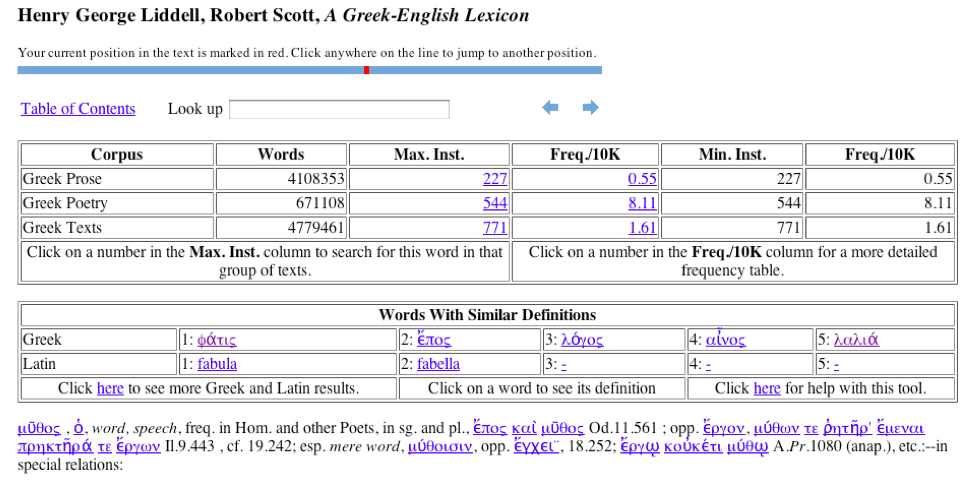
\includegraphics[width=\textwidth]{figure1.png}
			
			%\vspace{.125in}
			
			\caption{A screenshot of the Perseus 2.0 Dictionary Look-up, circa 2004, provided by Jeff Rydberg-Cox.  This shows the entry for μύθος.  The lower table, labelled “Words with similar definitions,” gives as synonyms the Greek words φάτις, ἔπος, λόγος, αἶνος, λαλιά, and the Latin words \textit{fabula} and \textit{fabella}.\label{perseussyns}}
		\end{figure}
		
	\section{Some new methods}
		
	\subsection{A new dictionary}
		
		At the same time, James Gawley brought a new dictionary to our attention, derived from \textbf{Whitaker's Words}\footnote{\url{http://users.erols.com/whitaker/words.htm}.  The plain-text version of the dictionary is here: \url{http://www.erols.com/whitaker/dictpage.zip}}.  At a glance, this dictionary seems to have entries for at least as many of the stems in our corpus as does the Perseus dictionary (given our current ability to parse it, anyway).  Each entry contains a simple and clearly marked English definition.  
		
		As we continue to develop a parser for the XML Lewis and Short, this new dictionary might allow us to develop matching algorithms on more clear-cut definitions.
		
	\subsection{A benchmark synonym set}
	
		I propose using \emph{Döderlein's Hand-Book of Latin Synonyms}\footnote{Von Döderlein, Ludwig (1858) \emph{Döderlein's Hand-Book of Latin Synonyms}.  Translated by H.\ H.\ Arnold.  Andover: W. F. Draper.} as a benchmark for testing our synonym-detectors.  A PDF version of this 19th-century textbook is available from Google Books at \url{http://books.google.ca/books?id=ynYXAAAAYAAJ}.  While it's not perfect, it is mostly in English, and the Latin synonyms of each headword are pretty clearly indicated by the type, so it could probably be mined by an undergraduate intern.
		
		As an example of how we might use this, I randomly selected 10 entries from Döderlein and transcribed each headword and its synonyms.  Döderlein isn't saying these words are identical; in most cases he's giving detailed instructions on how to differentiate them.  Nevertheless, the fact that they appear together in one entry shows that they are semantically related.  It would at least be profitable for us to consider whether this relationship is the kind of thing we're looking for.
		
		I used a random number generator to choose the page, and again to choose the entry.  Where it redirected to another entry, I followed that redirection and used that headword and its synonyms as the synonyms of the word I'd originally looked up.  In a couple of cases a synonym was mentioned in the body of the entry that was not in the entry head.  These words were in double-spaced type, as were those synonyms which were listed in the head.  Such words were included along with the other synonyms.  In two cases, the form of the word in Döderlein was different from the lemma in Whitaker.  In one case, Döderlein used the plural (\textit{compedes}) and Whitaker the singular (\textit{compes}), and in the other they give different principal parts of the verb (Döderlein, \textit{perferre}, and Whitaker, \textit{perfero}).  I had to manually adjust Döderlein's in order to get the program to work.
		
		Table \ref{doderlein} gives the ten randomly selected entries.
		
		\begin{table}			
		\caption{benchmark words with synonyms from Döderlein\label{doderlein}}
		\vspace{.25in}
		\begin{tabular}{ll}
		\textbf{compedes}* & vincula, catenae, pedicae, manicae\\
		\textbf{eloquens} & disertus, facundus, eloquens\\
		\textbf{excellens} & eminens, praeclarus, praestans, insignis, singularis, unicus, egregius, eximius\\
		\textbf{faux} & glutus, ingluvies, guttur, gurgulio, gula\\
		\textbf{frugifer} & foecundus, fertilis, ferax, uber, fructuosus\\
		\textbf{jocus} & ludus, lusus, ludicrum\\
		\textbf{macer} & exilis, gracilis, tenuis\\
		\textbf{malignitas} & invidia, livor, invidentia, obtrectatio, detrectatio\\
		\textbf{ostium} & janua, fores, valvae\\
		\textbf{perferre}* & ferre, tolerare, perpeti, sustinere, sinere, sustentare, pati\\
		\end{tabular}

		\vspace{.125in}
		*these were changed manually to agree with Whitaker's \textit{compes} and \textit{perfero}.
		\end{table}
		
	\subsection{Topic modelling on the dictionary}
	
		I thought I'd try applying the topic modelling software that we're using in the Co-occurrence Approach to the Whitaker dictionary.  I'm using the Python package \textbf{gensim}, working through the tutorials at \url{http://radimrehurek.com/gensim/}. The default application for this software seems to be document retrieval.  I treated each English definition in the dictionary as a document, and the English definition of a given headword as a query.  The definitions which the program ranked most similar ought to belong to the closest synonyms.
		
		Each English entry was converted to lowercase and split into words; all non alpha characters were thrown out.  I removed any words that occurred only once, as well as any words that occurred more than 215 times.  This latter number is totally arbitrary; my idea was that function words wouldn't be very useful, and a brief glance at the most frequent words suggested most of the words occurring more than 215 times weren't important parts of the definitions, but it would probably be smart to fool around with this.
		
		Following the tutorial, I transformed the corpus of English definitions to a tf-idf model, then to an LSI model\footnote{see \url{http://radimrehurek.com/gensim/tut1.html}, \url{http://radimrehurek.com/gensim/tut2.html}}.  To compare the entries, I used cosine similarity, again following the online tutorial\footnote{\url{http://radimrehurek.com/gensim/tut3.html}}.  The range of this similarity index is -1 (least similar) to 1 (most similar).  In the results below, I give the top 25 results (which always include the headword I searched for as the closest match) along with their similarity scores.
		
	\section{Results}

	Tables \ref{compes}–\ref{perfero} give the 25 closest entries for each of the headwords looked up in Döderlein (see Table \ref{doderlein}).  The caption for each table gives the headword with Döderlein's synonyms.  The table gives the similarity metric for each result, along with an abbreviated form of Whitaker's entry.  
	
	The top row in each case is the entry for the headword I looked up.  By looking at the English definition in this row, you can see what the similarity measurement had to go on.  In some cases it's apparent that what seems like an inappropriate word was responsible for many of the top results—for example, “things” in Table \ref{compes}.
	
	\section{First impressions, further work}
	
	While it's clear that many of the top results are semantically related to the headword, the relationship between Döderlein's synonyms and the automatic results was very low.  This might say more about the validity of the benchmark set than that of the automatic detection algorithm, of course, but it's equally clear that the results include words that are not semantically related to the headword, or at least much less so than important words that don't appear in the list.
	
	For each of these queries, the program actually ranked every word in the dictionary.  My choice of the top 25 was arbitrary, and doesn't give us much of a sense of the range of the similarity metric.  The 25th term is rarely below .5 on the scale of -1 to 1, and frequently there are some terms which seem relevant near the bottom of the list.
	
	If we were going to cut this list off at some point, should it be at a certain similarity level?  After a maximum number of synonyms?  Jeff Rydberg-Cox used a maximum of 5 synonyms, but it seems clear, e.g.\ from Table \ref{eloquens}, that more may well be appropriate in some cases.  It would be interesting to measure the slope of the decline of the similarity metric for a large number of headwords.
	
	It would be exciting to try this approach on Lewis and Short.  It might be that gensim's topics are fuzzy enough to deal with a certain amount of noise in the definitions.
	
	Finally, I'd like to pursue wholesale, unsupervised clustering of all the entries, rather than just retrieving similarity measurements against one query at a time.  This ought to be possible, but I'm still working through the gensim tutorials.
	
	Meanwhile, we should definitely continue the original line of research in the Dictionary Approach.  Rydberg-Cox's success with what is basically the same or even a less-sophisticated method should encourage us to proceed with new heart.

	\begin{sidewaystable}
	\caption{\textbf{compes} : vincula, catenae, pedicae, manicae \label{compes}}
	\vspace{.25in}
	\begin{tabular}{l|lll}
	   0.998503 & compes & N (3rd) F & shackles (for feet) (usu. pl.), fetters; things impeding movement; chains;\\
	   0.998503 & conpes & N (3rd) F & shackles (for feet) (usu. pl.), fetters; things impeding movement; chains;\\
	   0.701839 & creatum & N (2nd) N & things made (pl.);\\
	   0.701246 & nomenclatura & N (1st) F & assigning of names to things, nomenclature; mentioning things by name;\\
	   0.700858 & agraphum & N (2nd) N & things (pl.) unwritten;\\
	   0.700204 & dejector & N (3rd) M & one who throws/casts (things) down;\\
	   0.695552 & carnale & N (3rd) N & carnal/sensual/worldly things; things of the flesh;\\
	   0.695545 & cosmicum & N (2nd) N & worldly things (pl.);\\
	   0.691006 & dictatum & N (2nd) N & things dictated (pl.); dictated lessons or exercises; lessons; precepts/rules;\\
	   0.690147 & contaminatum & N (2nd) N & adulterated/contaminated things (pl.);\\
	   0.689641 & descriptum & N (2nd) N & diary, journal; things (pl.) recorded, writings;\\
	   0.687927 & inanimale & N (3rd) N & lifeless/inanimate things (pl.);\\
	   0.687927 & inanimans & N (3rd) N & lifeless/inanimate things (pl.);\\
	   0.685218 & immemoratum & N (2nd) N & things (pl.) not told/related; things not mentioned;\\
	   0.685218 & inmemoratum & N (2nd) N & things (pl.) not told/related; things not mentioned;\\
	   0.681307 & creamen & N (3rd) N & elements of which created things consist;\\
	   0.680565 & corporaliter & ADV & in respect of material things; carnally; corporally, bodily (L+S);\\
	   0.679753 & volans & N (3rd) M & mercury (element); flying/soaring things, birds (pl.);\\
	   0.676361 & circumjacentium & N (2nd) N & context (pl.), things/material around;\\
	   0.672397 & fulgur & N (3rd) N & lightning, flashing, brightness; [pubica ~ => things blasted by lightning];\\
	   0.667108 & stolidus & ADJ & dull, stupid, insensible; brutish; inert (things);\\
	   0.666296 & amatrix & ADJ & amorous; (applied to things);\\
	   0.664694 & sutilis & ADJ & made by sewing, consisting of things stitched together;\\
	   0.661379 & buttubattum & N (2nd) N & trifles (pl.), worthless things (L+S) (decl. uncertain);\\
	\end{tabular}
	\end{sidewaystable}


	\begin{sidewaystable}
	\caption{\textbf{eloquens} : disertus, facundus, eloquens \label{eloquens}}
	\vspace{.25in}
	\begin{tabular}{l|lll}
	   0.998563 & eloquens & ADJ & eloquent, expressing thoughts fluently/forcefully; articulate, able in speech;;\\
	   0.966847 & contestatiuncula & N (1st) F & short speech;\\
	   0.966288 & facundus & ADJ & eloquent; fluent; able to express eloquently/fluently (speech/written);\\
	   0.966168 & acyrologia & N (1st) F & impropriety of speech;\\
	   0.965835 & oratiuncula & N (1st) F & little speech, short oration;\\
	   0.965814 & suaviloquentia & N (1st) F & sweetness of speech;\\
	   0.965195 & barbarismus & N (2nd) M & barbarism, impropriety of speech;\\
	   0.965068 & dialectos & N F & dialect; form of speech;\\
	   0.965068 & dialectus & N (2nd) F & dialect; form of speech;\\
	   0.965065 & breviloquentia & N (1st) F & brevity of speech, conciseness;\\
	   0.965065 & breviloquium & N (2nd) N & brevity of speech, conciseness;\\
	   0.961566 & loquela & N (1st) F & speech, utterance;\\
	   0.961566 & loquella & N (1st) F & speech, utterance;\\
	   0.957994 & defricate & ADV & sharply, keenly; (of speech); with biting sarcasm (L+S);\\
	   0.957678 & oratio & N (3rd) F & speech, oration; eloquence; prayer;\\
	   0.955877 & causidicatus & N (2nd) M & forensic oratory, pleading/speech of a lawyer;\\
	   0.955227 & salebra & N (1st) F & rut, irregularity; roughness (of style or speech);\\
	   0.953286 & schematismos & N M & florid/figurative mode of speech;\\
	   0.953286 & schematismus & N (2nd) M & florid/figurative mode of speech;\\
	   0.950448 & actiuncula & N (1st) F & short judicial harangue; unimportant speech;\\
	   0.94659 & blaesus & ADJ & lisping, stammering; indistinct; mispronouncing from speech defect/drunkenness;\\
	   0.941469 & libertas & N (3rd) F & freedom, liberty; frankness of speech, outspokenness;\\
	   0.940028 & parabola & N (1st) F & comparison; explanatory illustration; parable (L+S), allegory; proverb; speech;\\
	   0.940028 & parabole & N F & comparison; explanatory illustration; parable (L+S), allegory; proverb; speech;\\
	\end{tabular}
	\end{sidewaystable}


	\begin{sidewaystable}
	\caption{\textbf{excellens} : eminens, praeclarus, praestans, insignis, singularis, unicus, egregius, eximius \label{excellens}}
	\vspace{.25in}
	\begin{tabular}{l|lll}
	   0.999927 & excellens & ADJ & distinguished, excellent;\\
	   0.994202 & praecellens & ADJ & surpassing, excellent, distinguished; preeminent;\\
	   0.949481 & egregius & ADJ & singular; distinguished; exceptional; extraordinary; eminent; excellent;\\
	   0.932508 & superexcellens & ADJ & very excellent;\\
	   0.776643 & adprobus & ADJ & excellent, worthy;\\
	   0.776643 & approbus & ADJ & excellent, worthy;\\
	   0.765041 & praestabilis & ADJ & pre-eminent, superior; distinguished, excellent;\\
	   0.7147 & dapaticus & ADJ & splendid/excellent; sumptuous/magnificent/stately; noble/eminent; proud/boastful\\
	   0.7147 & magnificus & ADJ & splendid/excellent/sumptuous/magnificent/stately; noble/eminent; proud/boastful;\\
	   0.7147 & magnuficus & ADJ & splendid/excellent/sumptuous/magnificent/stately; noble/eminent; proud/boastful;\\
	   0.67824 & eximius & ADJ & select; extraordinary/special; excellent; [Doctor Eximius => Francis Suarez];\\
	   0.668614 & honestus & ADJ & distinguished, reputable, respected, honorable, upright, honest; worthy;\\
	   0.659768 & circumspectus & ADJ & |worthy of consideration, respected; distinguished;\\
	   0.548678 & perdignus & ADJ & very worthy;\\
	   0.546617 & condemnabilis & ADJ & worthy of condemnation;\\
	   0.54586 & damnabilis & ADJ & damnable, worthy of condemnation/damnation;\\
	   0.540548 & differens & ADJ & different; superior; excellent;\\
	   0.539146 & adorabilis & ADJ & adorable, worthy of adoration/veneration;\\
	   0.539146 & adorandus & ADJ & adorable, worthy of adoration/veneration;\\
	   0.528756 & consulariter & ADV & in a manner befitting/worthy of a consul;\\
	   0.524033 & amphitheatralis & ADJ & of/in the amphitheater; worthy of the amphitheater;\\
	   0.522355 & aspernabilis & ADJ & contemptible, negligible; worthy to be disdained, such as might be disdained;\\
	   0.52026 & cantabilis & ADJ & worthy to be sung;\\
	   0.509952 & dignabilis & ADJ & worthy, deserving, meriting;\\
	\end{tabular}
	\end{sidewaystable}


	\begin{sidewaystable}
	\caption{\textbf{faux} : glutus, ingluvies, guttur, gurgulio, gula \label{faux}}
	\vspace{.25in}
	\begin{tabular}{l|lll}
	   0.993435 & faux & N (3rd) F & pharynx (usu pl.), gullet/throat/neck/jaws/maw; narrow pass/shaft/strait; chasm;\\
	   0.699992 & saltus & N (4th) M & narrow passage (forest/mountain); defile, pass; woodland with glades (pl.);\\
	   0.693242 & deveho & V (3rd) TRANS & |descend, go down (PASS); go away;\\
	   0.691022 & adlicefio & V SEMIDEP & be/become enticed/allured/lured; (allicefacio PASS);\\
	   0.691022 & allicefio & V SEMIDEP & be/become enticed/allured/lured; (allicefacio PASS);\\
	   0.690835 & benefio & V SEMIDEP & be blessed; receive a benefit; (benefacio PASS);\\
	   0.690529 & malefio & V SEMIDEP & be injured; (malefacio PASS);\\
	   0.689334 & abolefio & V SEMIDEP & be destroyed; (abolefacio PASS);\\
	   0.688914 & cavefio & V SEMIDEP & be avoided; be stipulated; (cavefacio PASS);\\
	   0.687897 & deponefio & V SEMIDEP & be deposited/put down; (deponefacio PASS);\\
	   0.68635 & consuefio & V SEMIDEP & be/become accustomed/acclimated/habituated/hardened (to); (consuefacio PASS);\\
	   0.685236 & praetermitto & V (3rd) & let pass; pass over; omit; overlook;\\
	   0.683587 & condocefio & V SEMIDEP & be/become trained/disciplined/taught/instructed (L+S); (condocefacio PASS);\\
	   0.683052 & labefio & V SEMIDEP & be made unsteady; be loosened/shaken; be subverted; (labefacio PASS);\\
	   0.682952 & stupefio & V SEMIDEP & be stunned (w/amazement), be stupefied/struck senseless; (stupefacio PASS);\\
	   0.68235 & expergefio & V SEMIDEP & be awakened/aroused/excited; (expergefacio PASS);\\
	   0.682112 & commonefio & V SEMIDEP & be recalled/remembered/reminded; be warned/admonished; (commonefacio PASS);\\
	   0.682112 & conmonefio & V SEMIDEP & be recalled/remembered/reminded; be warned/admonished; (conmonefacio PASS);\\
	   0.681754 & circummeo & V (1st) & go/travel/pass around;\\
	   0.681131 & adsuefio & V SEMIDEP & be/become accustomed (to), be habituated; be trained; (adsuefacio PASS);\\
	   0.681131 & assuefio & V SEMIDEP & be/become accustomed (to), be habituated; be trained; (assuefacio PASS);\\
	   0.678961 & fabrefio & V SEMIDEP & be made or fashioned skillfully; (fabrefacio PASS);\\
	   0.677655 & obstupefio & V SEMIDEP & be astonished/dazed/paralyzed/stunned (w/emotion); (obstupefacio PASS);\\
	   0.676887 & tabefio & V SEMIDEP & be melted/dissolved/subdued; (tabefacio PASS);\\
	\end{tabular}
	\end{sidewaystable}


	\begin{sidewaystable}
	\caption{\textbf{frugifer} : foecundus, fertilis, ferax, uber, fructuosus \label{frugifer}}
	\vspace{.25in}
	\begin{tabular}{l|lll}
	   0.999311 & frugifer & ADJ & fruit-bearing, fertile;\\
	   0.999239 & fructifer & ADJ & fruitful; fruit-bearing, bearing fruit;\\
	   0.996636 & fructuarius & ADJ & fruit-bearing, fruitful;\\
	   0.992159 & pomifer & ADJ & fruit-bearing;\\
	   0.97206 & auctifer & ADJ & productive, fruitful, fertile; fruit-bearing (L+S);\\
	   0.956114 & conifer & ADJ & coniferous, cone-bearing (tree); bearing fruit of a conical form (L+S);\\
	   0.956114 & coniger & ADJ & coniferous, cone-bearing (tree); bearing fruit of a conical form (L+S);\\
	   0.925968 & fetus & N (4th) M & |||fruit of plant; produce/crop; offshoot/branch/sucker/sapling; bearing fruit;\\
	   0.925968 & foetus & N (4th) M & |||fruit of plant; produce/crop; offshoot/branch/sucker/sapling; bearing fruit;\\
	   0.893095 & bifer & ADJ & bearing twice, bearing fruit or flowers twice a year;\\
	   0.865896 & malifer & ADJ & apple-bearing;\\
	   0.842441 & sementifer & ADJ & seed-bearing, fruitful;\\
	   0.810886 & ostrifer & ADJ & bearing oysters;\\
	   0.810387 & glandifer & ADJ & acorn-bearing;\\
	   0.809803 & baccifer & ADJ & berry-bearing;\\
	   0.809803 & bacifer & ADJ & berry-bearing;\\
	   0.809696 & palmifer & ADJ & palm-bearing;\\
	   0.80715 & sceptrifer & ADJ & bearing a scepter;\\
	   0.806667 & salutigerulus & ADJ & greetings-bearing;\\
	   0.806276 & coruscifer & ADJ & lightening-bearing;\\
	   0.806118 & racemifer & ADJ & bearing clusters;\\
	   0.801846 & bipennifer & ADJ & bearing a two edged axe;\\
	   0.801831 & defloreo & V (2nd) INTRANS & drop/shed blossoms/petals (before bearing fruit);\\
	   0.801821 & gemellipara & N (1st) F & twin-bearing;\\
	\end{tabular}
	\end{sidewaystable}


	\begin{sidewaystable}
	\caption{\textbf{jocus} : ludus, lusus, ludicrum \label{jocus}}
	\vspace{.25in}
	\begin{tabular}{l|lll}
	   0.999938 & jocus & N (2nd) M & joke, jest; sport;\\
	   0.937306 & jocatio & N (3rd) F & joke, jest;\\
	   0.937306 & joculor & V (1st) DEP & jest; joke;\\
	   0.937306 & ridiculare & N (3rd) N & jest, joke (as pl.);\\
	   0.888865 & methodium & N (2nd) N & trick, artifice; jest, joke (L+S);\\
	   0.868856 & joco & V (1st) & joke, jest; say in jest; make merry;\\
	   0.868856 & jocor & V (1st) DEP & joke, jest; say in jest; make merry;\\
	   0.855803 & facetia & N (1st) F & wit (pl.), joke;\\
	   0.804608 & dicterium & N (2nd) N & joke, witticism; witty saying (L+S); bon mot;\\
	   0.681826 & dictabolarium & N (2nd) N & joke (pl.); (nonce-word indicating verbal joke); satirical saying (L+S);\\
	   0.639222 & logos & N M & word; mere words (pl.), joke, jest, bon mot;\\
	   0.639222 & logus & N (2nd) M & word; mere words (pl.), joke, jest, bon mot;\\
	   0.587207 & nartatio & N (3rd) F & skiing (sport);\\
	   0.556579 & athletica & N (1st) F & athletics; sport;\\
	   0.54947 & ridiculum & N (2nd) N & joke, piece of humor; [per ridiculum => jockingly, for fun];\\
	   0.484541 & adludo & V (3rd) & frolic/play/sport around/with, play against; jest, make mocking allusion to;\\
	   0.484541 & alludo & V (3rd) & frolic/play/sport around/with, play against; jest, make mocking allusion to;\\
	   0.481977 & catampo & N (3rd) C & kind of play/sport/game;\\
	   0.479943 & ludo & V (3rd) & play, mock, tease, trick;\\
	   0.427897 & adludio & V (1st) INTRANS & play/frolic (with);\\
	   0.427897 & alludio & V (1st) INTRANS & play/frolic (with);\\
	   0.427326 & satyrus & N (2nd) M & satyr; satyric play;\\
	   0.425582 & analogicus & ADJ & analogous; of grammatical analogy/similarity (word inflections/derivations);\\
	   0.423418 & ludus & N (2nd) M & game, play, sport, pastime, entertainment, fun; school, elementary school;\\
	\end{tabular}
	\end{sidewaystable}


	\begin{sidewaystable}
	\caption{\textbf{macer} : exilis, gracilis, tenuis \label{macer}}
	\vspace{.25in}
	\begin{tabular}{l|lll}
	   0.999182 & macer & ADJ & thin (men, animals, plants), scraggy, lean, small, meager; thin (soil), poor;\\
	   0.790526 & macilentus & ADJ & thin, lean; meager (L+S);\\
	   0.788139 & exilis & ADJ & small, thin; poor;\\
	   0.768003 & depugis & ADJ & having meager/skinny/thin buttocks;\\
	   0.768003 & depygis & ADJ & having meager/skinny/thin buttocks;\\
	   0.757342 & runco & V (1st) TRANS & weed, thin out;\\
	   0.756582 & crocotillus & ADJ & very thin;\\
	   0.755826 & extenuo & V (1st) & make thin; diminish;\\
	   0.754225 & vescus & ADJ & thin, attenuated;\\
	   0.747168 & levidensis & ADJ & thin, slight, poor;\\
	   0.733036 & pertenuis & ADJ & very thin; very slender;\\
	   0.725648 & praetenuis & ADJ & very thin; very slender; very shrill;\\
	   0.721975 & resticula & N (1st) F & thin rope;\\
	   0.689155 & generositas & N (3rd) F & breeding, excellence/nobility (of stock/men/animals/plants); generosity;\\
	   0.66573 & petilus & ADJ & thin; slender (archaic);\\
	   0.655893 & diraro & V (1st) TRANS & thin out (vegetation); chop, hoe;;\\
	   0.655893 & disraro & V (1st) TRANS & thin out (vegetation); chop, hoe;;\\
	   0.647855 & funiculus & N (2nd) M & thin rope, cord, string;\\
	   0.642856 & adtenuo & V (1st) TRANS & thin (out); weaken, lessen, diminish, shrink, reduce in size; make plain;\\
	   0.642856 & attenuo & V (1st) TRANS & thin (out); weaken, lessen, diminish, shrink, reduce in size; make plain;\\
	   0.639766 & tenuo & V (1st) & make thin; reduce, lessen; wear down;\\
	   0.637559 & adrigo & V (1st) TRANS & water (plants), moisten the soil around;\\
	   0.637559 & arrigo & V (1st) TRANS & water (plants), moisten the soil around;\\
	   0.633367 & trama & N (1st) F & warp (weaving); woof, weft, web filling; thin/lank figure; trifles; bagatelles;\\
	\end{tabular}
	\end{sidewaystable}


	\begin{sidewaystable}
	\caption{\textbf{malignitas} : invidia, livor, invidentia, obtrectatio, detrectatio \label{malignitas}}
	\vspace{.25in}
	\begin{tabular}{l|lll}
	   0.999865 & malignitas & N (3rd) F & ill-will, spite, malice; niggardliness;\\
	   0.979007 & malitia & N (1st) F & ill will, malice; wickedness; vice, fault;\\
	   0.964156 & malevolentia & N (1st) F & ill-will/spite/malice; malevolence; dislike/hatred/envy (L+S); evil disposition;\\
	   0.964156 & malivolentia & N (1st) F & ill-will/spite/malice; malevolence; dislike/hatred/envy (L+S); evil disposition;\\
	   0.945942 & invideo & V (2nd) & envy, regard with envy/ill will; be jealous of; begrudge, refuse;\\
	   0.871725 & intempestivus & ADJ & untimely, ill timed; unreasonable;\\
	   0.870287 & inconvenienter & ADV & unsuitably; ill-matchedly; inconveniently;\\
	   0.86919 & malesuadus & ADJ & ill-advising;\\
	   0.867853 & inconsultus & ADJ & rash, ill-advised, thoughtless, injudicious; unconsulted, not asked;\\
	   0.864944 & immerens & ADJ & undeserving (of ill treatment), blameless;\\
	   0.862596 & indigne & ADV & |dishonorably (L+S); indignantly; [~ fero => be indignant at; resent/take ill];\\
	   0.858086 & minax & ADJ & threatening; boding ill;\\
	   0.848684 & obscaenus & ADJ & |inauspicious/unpropitious; ill-omened/boding ill; filthy, polluted, disgusting;\\
	   0.848684 & obscenus & ADJ & |inauspicious/unpropitious; ill-omened/boding ill; filthy, polluted, disgusting;\\
	   0.848684 & opscaenus & ADJ & |inauspicious/unpropitious; ill-omened/boding ill; filthy, polluted, disgusting;\\
	   0.848684 & opscenus & ADJ & |inauspicious/unpropitious; ill-omened/boding ill; filthy, polluted, disgusting;\\
	   0.836981 & malevolus & ADJ & spiteful, malevolent; ill-disposed; disaffected (L+S); envious;\\
	   0.836981 & malivolens & ADJ & spiteful, malevolent; ill-disposed; disaffected (L+S); envious;\\
	   0.836981 & malivolus & ADJ & spiteful, malevolent; ill-disposed; disaffected (L+S); envious;\\
	   0.834593 & invidentia & N (1st) F & jealousy, envy;\\
	   0.82956 & invidus & ADJ & hateful, ill disposed, hostile, malevolent; envious, jealous, grudging;\\
	   0.828967 & monstruosus & ADJ & strange, monstrous, ill-omened;\\
	   0.823228 & gannitus & N (4th) M & yelping/snarling/barking; ill-tempered utterance; whimpering/whining/moaning;\\
	   0.813525 & stomachus & N (2nd) M & gullet; stomach; annoyance; ill-temper;\\
	\end{tabular}
	\end{sidewaystable}


	\begin{sidewaystable}
	\caption{\textbf{ostium} : janua, fores, valvae \label{ostium}}
	\vspace{.25in}
	\begin{tabular}{l|lll}
	   0.999151 & ostium & N (2nd) N & doorway; front door; starting gate; entrance (underworld); (river) mouth;\\
	   0.962876 & austium & N (2nd) N & door (w/frame); front door; starting gate; entrance to underworld; river mouth;\\
	   0.757137 & Stygius & ADJ & Stygian; of the river Styx; of the underworld;\\
	   0.752552 & Styx & N F & Styx river; river of the underworld;\\
	   0.749808 & egressus & N (4th) M & landing place; egress; departure; flight; landing; mouth (of a river);\\
	   0.744135 & Padus & N (2nd) M & Po river;\\
	   0.74238 & fluvialis & ADJ & river;\\
	   0.74238 & fluviaticus & ADJ & river-; of a river;\\
	   0.74238 & Indus & N (2nd) M & Indus (river);\\
	   0.7421 & Euphrates & N (3rd) M & Euphrates; (river);\\
	   0.741508 & barbus & N (2nd) M & barbel, river barbel (Cyprinus barbus);\\
	   0.740511 & Albis & N (3rd) M & Elbe; (river in Germany);\\
	   0.735701 & ripensis & ADJ & on river-bank;\\
	   0.731552 & Mosa & N (1st) F & river Maas/Meuse, in Holland/France/Belgium;\\
	   0.729242 & stygius & ADJ & Stygian, of river Styx; of fountain Styx;\\
	   0.720398 & alluvies & N (5th) F & silt, soil deposited by a river; floodland by a river; lapping of waves;\\
	   0.716989 & amnicolus & ADJ & growing beside a river (-a, -ae for M/F); dwelling beside a river (L+S);\\
	   0.715787 & adluvius & ADJ & alluvial, from river overflow/deposit;\\
	   0.715787 & alluvius & ADJ & alluvial, from river overflow/deposit;\\
	   0.715443 & Tiberis & N (3rd) C & Tiber; (the river at Rome);\\
	   0.712582 & portula & N (1st) F & little gate, postern;\\
	   0.712562 & amnis & N (3rd) M & river (real/personified), stream; current; (running) water; the river Ocean;\\
	   0.705146 & littus & N (3rd) N & shore, seashore, coast, strand; river bank; beach, landing place;\\
	   0.705146 & litus & N (3rd) N & shore, seashore, coast, strand; river bank; beach, landing place;\\
	\end{tabular}
	\end{sidewaystable}


	\begin{sidewaystable}
	\caption{\textbf{perfero} : ferre, tolerare, perpeti, sustinere, sinere, sustentare, pati \label{perfero}}
	\vspace{.25in}
	\begin{tabular}{l|lll}
	   0.998084 & perfero & V & carry through; bear, endure to the end, suffer; announce;\\
	   0.812086 & perpetro & V (1st) & carry through, accomplish;\\
	   0.807455 & perago & V (3rd) & disturb; finish; kill; carry through to the end, complete;\\
	   0.795573 & executo & V (3rd) TRANS & |execute, carry out (duty); go through, rehearse; pursue; develop (topic);\\
	   0.795573 & exsecuto & V (3rd) TRANS & |execute, carry out (duty); go through, rehearse; pursue; develop (topic);\\
	   0.743877 & adtulo & V (3rd) TRANS & bring/carry/bear to;\\
	   0.743877 & attulo & V (3rd) TRANS & bring/carry/bear to;\\
	   0.743877 & circumgesto & V (1st) TRANS & carry/bear about/around;\\
	   0.741102 & baijulo & V (1st) TRANS & carry, bear (load);\\
	   0.741102 & bajulo & V (1st) TRANS & carry, bear (load);\\
	   0.733308 & gesto & V (1st) & bear, carry; wear;\\
	   0.725815 & egero & V (3rd) & carry or bear out, discharge, utter;\\
	   0.688963 & perveho & V (3rd) & bear, carry or convey through; [pervehi, pass =>  to sail to, ride to];\\
	   0.677657 & ursinus & ADJ & bear-; of a bear;\\
	   0.677657 & ursus & N (2nd) M & bear;\\
	   0.675263 & gero & V (3rd) & bear, carry, wear; carry on; manage, govern; (se gerere = to conduct oneself);\\
	   0.66155 & suffero & V & bear, endure, suffer;\\
	   0.655159 & tolero & V (1st) & bear, endure, tolerate;\\
	   0.640318 & exequor & V (3rd) DEP & |persist in; execute, carry out; rehearse; attain, arrive at, accomplish;\\
	   0.640318 & exsequor & V (3rd) DEP & |persist in; execute, carry out; rehearse; attain, arrive at, accomplish;\\
	   0.630674 & elimino & V (1st) & carry out of doors; [w/dicta => to blab];\\
	   0.630303 & congesto & V (1st) TRANS & bring/carry together;\\
	   0.630303 & devecto & V (1st) TRANS & carry away;\\
	   0.630303 & porto & V (1st) & carry, bring;\\
	\end{tabular}
	\end{sidewaystable}

\end{document}
